\documentclass[hyperref={colorlinks=true},xcolor=svgnames]{beamer}
\usepackage{pgfpages}
\usepackage{listings}
\usepackage{amsmath} 
\setbeamercolor{normal text}{bg=BlanchedAlmond}



\mode<presentation>
{
  \usetheme{Pittsburgh}
  \useoutertheme[right]{sidebar}
  % or ...

  \setbeamercovered{transparent}
  % or whatever (possibly just delete it)
}


\usepackage[english]{babel}
\usepackage{listings}

\usepackage[latin1]{inputenc}


\usepackage{times}
\usepackage[T1]{fontenc}
\usepackage{xcolor}


\def \lecturenumber {1}
\newcommand*\oldmacro{}
\let\oldmacro\insertshortauthor% save previous definition
\renewcommand*\insertshortauthor{%
  \leftskip=.3cm% before the author could be a plus1fill ...
 \lecturenumber :  \insertframenumber\,/\,\inserttotalframenumber\hfill\oldmacro}

\title{Topic 1: Introduction, Vectors}

\AtBeginSubsection[]
{
  \begin{frame}<beamer>
    \frametitle{Outline}
    \tableofcontents[currentsection,currentsubsection]
  \end{frame}
 }

\usepackage{amssymb}
\usepackage{amsmath}

\usepackage{bm}
\newcommand{\catop}{\mbox{}^\frown}
\renewcommand{\v}[1]{\underline{#1}}
\newcommand{\vt}[1]{\underline{#1}^\intercal}
\newcommand{\uv}[1]{\underline{\hat{#1}}}
\newcommand{\vd}[2]{\begin{pmatrix}#1 \\ #2 \end{pmatrix}}
\newcommand{\vdt}[2]{\begin{pmatrix}#1 & #2 \end{pmatrix}}
\newcommand{\vdthree}[3]{\begin{pmatrix}#1 \\ #2 \\ #3 \end{pmatrix}}
\newcommand{\length}[1]{|\v{#1}|}
\renewcommand{\dot}[2]{{\v{#1}^\intercal} \cdot {\v{#2}}}
\newcommand{\matr}[1]{\mathbf{#1}}  
\newcommand{\invmatr}[1]{\matr{#1}^{-1}}
\newcommand{\transpose}[1]{\matr{#1}^{\intercal}}
\newcommand{\Identity}{\matr{I}}

\newcommand{\xdownarrow}[1]{%
  {\left\downarrow\vbox to #1{}\right.\kern-\nulldelimiterspace}
}
\newcommand{\xuparrow}[1]{%
  {\left\uparrow\vbox to #1{}\right.\kern-\nulldelimiterspace}
}



\newcommand{\pspiccie}[2]{
\centerline{\hskip0.1cm\setlength\epsfxsize{#2cm}\epsfbox{../Figures/#1}}}
\newcommand{\smallpspiccie}[1]{
\centerline{\hskip0.1cm\setlength\epsfxsize{6.0cm}\epsfbox{../Figures/#1}}}

\newcommand{\fullpara}[4]{
#1 \; \mbox{}_{#2} \|_{#3} \; #4}
\newcommand{\para}[2]{
#1 \; \ \| \; #2}

\newcommand{\socrative}{
\begin{frame}{Exercise}

GO TO socrative.com NOW

\end{frame}
}


\newcommand{\socr}[1]{
\begin{frame}{Exercise}

Go to the moodle page now.

\vskip2cm
\hfill{\tiny{#1}}

\end{frame}
}

\newcommand{\survey}[1]{
\begin{frame}{Exercise}

GO TO \url{#1} NOW


\end{frame}
}


\newcounter{topic}
\renewcommand{\theequation}{\thesection.\arabic{equation}}
\renewcommand{\thesection}{\arabic{topic}}






\setcounter{topic}{1}


\begin{document}

\begin{frame}
  \titlepage
\end{frame}

\section{Preamble}
\begin{frame}
\frametitle{Downloads}
\begin{itemize}
\item
All details for this course can be found on Moodle

\item
\url{http://moodle.rhul.ac.uk/}

\item
I will attempt to create a slidecast of each lecture that will be placed on moodle as well.
\end{itemize}

\end{frame}

\begin{frame}{Who am I ?}
\begin{itemize}
\item
Hugh Shanahan (but you can call me Hugh).

\item 
My office is in the Bedford Building. 

\item
Here are my office hours - please come by the admin office and ask them to give me a call.

\item Monday 15-16

\item Tuesday 15-16

\item 
If you want some guaranteed time with me to answer question etc., 
please email me to arrange an appointment. 
% My email address is 
%{\tt Hugh.Shanahan@rhul.ac.uk}.
\end{itemize}
\end{frame}

\begin{frame}
\frametitle{Assignments}
\begin{itemize}
\item 
Three quizzes - each worth 10\% of the final grade. 

\item 
Each quiz will be 30 minutes in length so it can be done in an hour slot.

\item A practice quiz will be set up this week.

\item 
Deadlines are available on 

%\url{https://www.royalholloway.ac.uk/computerscience/informationforcurrentstudents/home.aspx}



\end{itemize}
\end{frame}

\begin{frame}
\frametitle{Exam}

\begin{itemize}
%\item
%This is a new course and there will be an example exam script before the end of the course.
%
%\pause 

\item
Answer all questions !
\end{itemize}

\end{frame}

\begin{frame}
\frametitle{Labs}

\begin{itemize}
\item Labs will run on a weekly basis.

%\item Two hours once a fortnight.

\item Thursday 10-12, Bedford 0-04 to 0-0.06, PC01.

\item Class will be divided into two; each one taking one hour. 

\item No lab this week.

\item We'll be using Python and NumPy for this course.

\item More specifically we will be using Jupyter notebooks and Binder.
%\item First exercise - have a read of your First Year Games notes!!!

\end{itemize}

\end{frame}
\section{Motivation}
\begin{frame}
\frametitle{Motivation}

\begin{itemize}
\item This course will focus on one, very regular class of data structures.

\pause

\item Namely, vectors and matrices with almost invariably floating point entries.

\item Linear Algebra is the branch of Mathematics to deal with this.

\pause

\item Why bother??
 
\end{itemize}

\end{frame}

\begin{frame}
\frametitle{Linear Algebra}

\begin{itemize}
\item Linear Algebra is a vast branch of Mathematics with hugely powerful tools for us to use. 

\item Linear Algebra has a number of direct applications in Computer Science and every Computer Scientist should understand it. For example
\pause
\begin{itemize}
\item Computer Graphics
\item Computer Vision
\item Machine Learning and Artificial Intelligence
\item Graph Theory
\end{itemize}
\end{itemize}

\end{frame}

\begin{frame}
\frametitle{Mathematics}
\begin{itemize}
\item This course is shamelessly Mathematical BUT

\pause

\item I assume no prior knowledge of Linear Algebra.

\item It is very much grounded in concrete examples from CS. 
\end{itemize}


\end{frame}
\section{Definitions and Background Mathematics}

\begin{frame}
\frametitle{Definitions}

\begin{table}[htdp]

\begin{center}
\begin{tabular}{|c|c|c|}
\hline 
Type & Symbol & Examples \\ \hline
Natural numbers & $\mathbb{N}$ & $0$,$1$,$2$,$\dots$ \\ 
Integers & $\mathbb{Z}$ & $\dots$,$-2$,$-1$,$0$,$1$,$2$,$\dots$ \\ 
Reals & $\mathbb{R}$ & $-\pi$,$0$, $e$, $100.03$ \\
Complex numbers & $\mathbb{C}$ &$3.0 + 4.95 i$ \\ \hline 
\end{tabular}
\end{center}
\caption{Symbols used in this course.}
\label{Symbols}
\end{table}%


\end{frame} 

\begin{frame}
\frametitle{Notation}

\begin{table}[htdp]

\begin{center}
\begin{tabular}{|c|c|}
\hline 
Symbol & Meaning  \\ \hline
$\equiv$ & Defines \\
$\implies$ & This Implies \\
iff & If and Only if \\ \hline 
\end{tabular}
\end{center}
\caption{Notation used in this course.}
\label{Notation}
\end{table}%


\end{frame} 

\begin{frame}
\frametitle{Trigonometry}

%Quick reminder 

\begin{center}
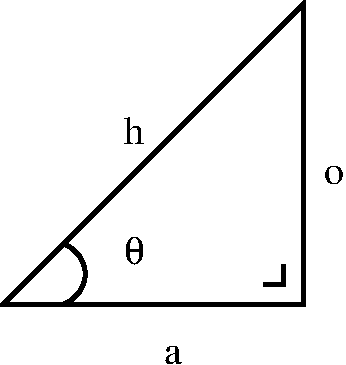
\includegraphics[height=3cm]{../Figures/Topic1_preamble.png}
\end{center}

\begin{eqnarray}
\cos{\theta} = \frac{a}{h} \;\; &, &
\sin{\theta} = \frac{o}{h} \;\; , \\
\cos{(-\theta)} = \cos \theta \;\; &,&
\sin{(-\theta)} = -\sin \theta \;\; \\
\cos^2{\theta} + \sin^2{\theta} &=& 1 \;\; , \\
\sin{(a+b)} &=& \sin{a} \cos{b} + \cos{a}\sin{b} \;\; , \\
\cos{(a+b)} &=& \cos{a} \cos{b} - \sin{a} \sin{b} \;\; .   
\end{eqnarray}




\end{frame}

\section{The number line}

\begin{frame}
\frametitle{The number line}

First steps in understanding numbers ($\mathbb{Z}$).

\vskip1cm
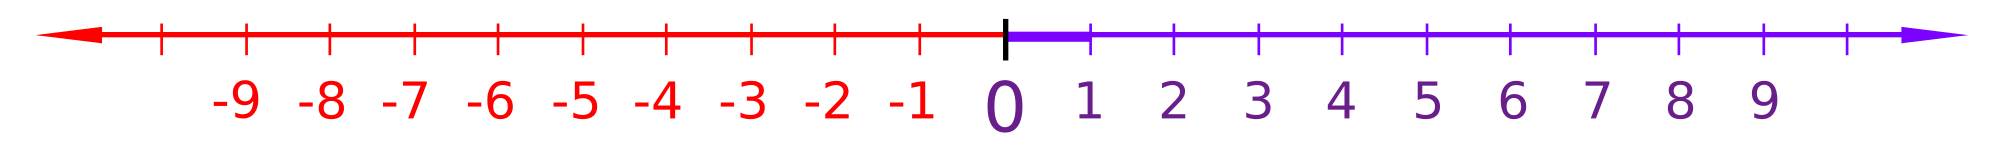
\includegraphics[height=0.75cm]{../Figures/2000px-Number-line.png}


\end{frame}

\begin{frame}
\frametitle{The reals}

Can add in reals easily in this picture $\dots$ ($\mathbb{R}$).

\vskip1cm
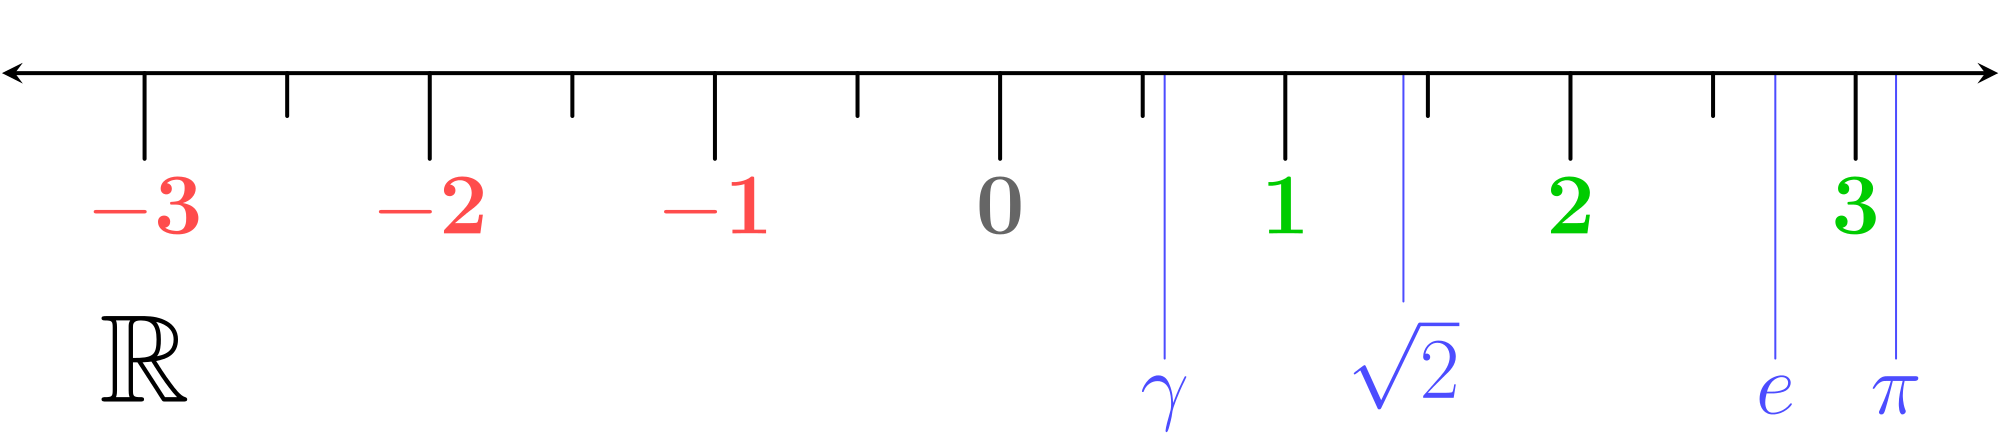
\includegraphics[height=2cm]{../Figures/Real_Number_line.png}


\end{frame}

\begin{frame}
\frametitle{Direction}

Can think of an arrow  from the origin to each  number on the number line.
\vskip1cm
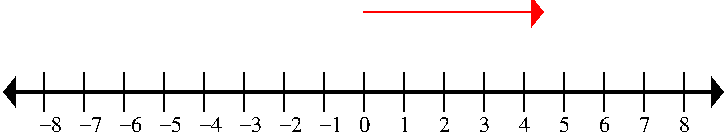
\includegraphics[height=1.5cm]{../Figures/1dvector.png}

Arrow is length 4.5 going in a positive direction. 

\end{frame}


\begin{frame}
\frametitle{Direction}


\vskip1cm
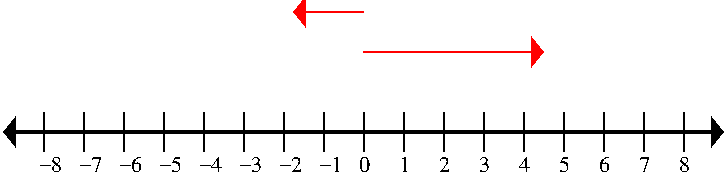
\includegraphics[height=1.5cm]{../Figures/1dvectorExample2.png}

Other arrow is length 1.66 going in a negative direction. 

\end{frame}

\begin{frame}
\frametitle{Operations - scaling}

Can scale the length of an arrow.
 
\vskip1cm
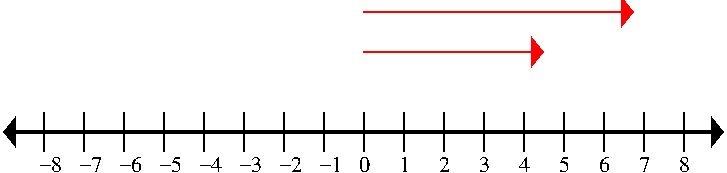
\includegraphics[height=1.5cm]{../Figures/1dvectorScaled.png}

Arrow of length 4.5 is scaled by a factor 1.5.

\end{frame}

\begin{frame}
\frametitle{Operations - addition}

Can add arrows - just put "tail to head". 
 
\vskip1cm
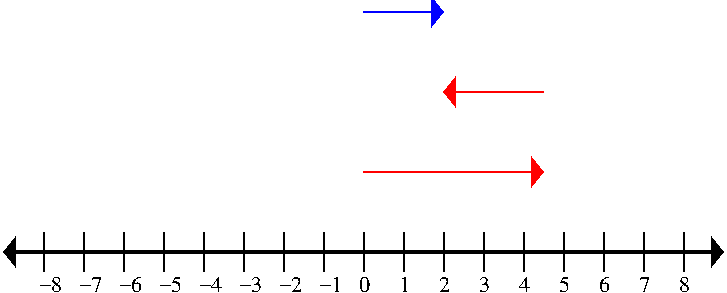
\includegraphics[height=1.5cm]{../Figures/1dvectorAddition.png}

Arrow of length 4.5 going in positive direction plus arrow of length 2.5 going in a negative direction results in an arrow of length 2.0 going in a 
positive direction. 

\end{frame}

\begin{frame}
\frametitle{Operations - product}

Multiplying the signs tells us if the arrows are going in the same or opposite direction. 

\end{frame}

\section{Two dimensions}

\begin{frame}
\frametitle{Adding another number line}

Move into 2 dimensions.

\vskip1cm
\begin{center}
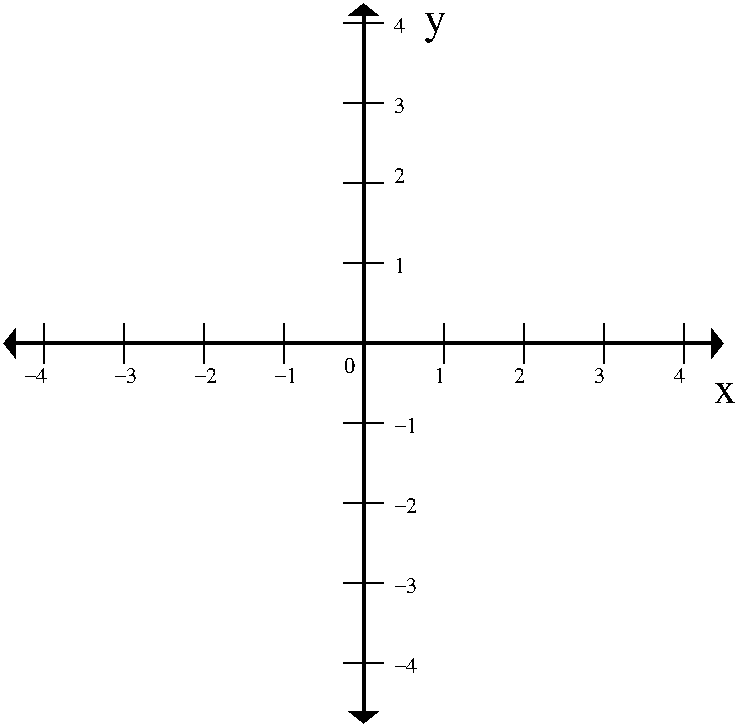
\includegraphics[height=6cm]{../Figures/2DGrid.png}
\end{center}

\end{frame}


\begin{frame}
\frametitle{Moving up a dimension}
\begin{itemize}
\item Instead of a position on the number line. You now have {\bf coordinates}, 
represented by a pair of numbers $(a,b)$. 
\pause
\item For the most part we will assume that these numbers are reals $a \in \mathbb{R}$, 
$b \in \mathbb{R}$.
\pause
\item Formally, these are elements of the Cartesian product $\mathbb{R} \times \mathbb{R}$
(go and check your CS1860 notes). 
\pause
\item But we could have grids which are  $\mathbb{N} \times \mathbb{N}$, 
$\mathbb{Z} \times \mathbb{Z}$, $\mathbb{C} \times \mathbb{C}$ 
and so on. 
\end{itemize}
\end{frame}

\begin{frame}
\frametitle{A coordinate}

\vskip1cm
\begin{center}
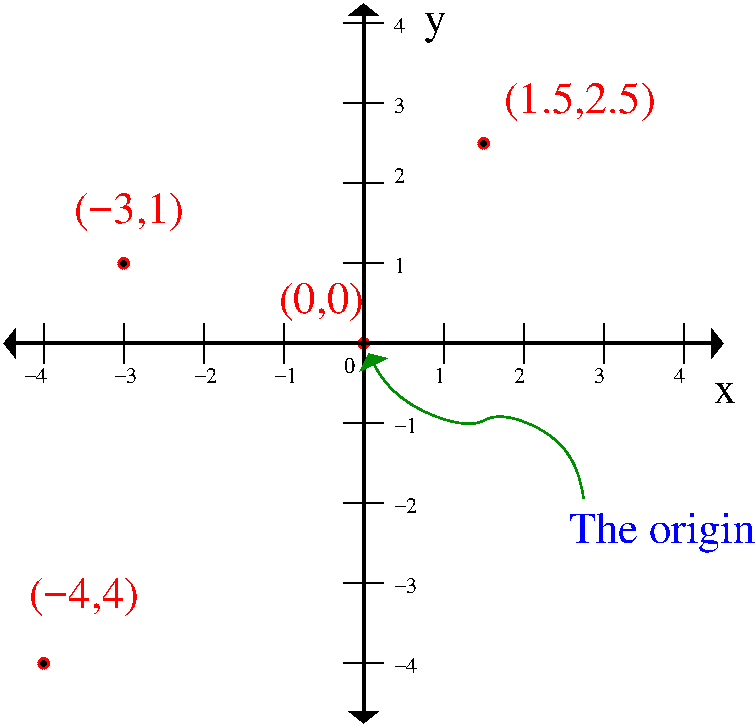
\includegraphics[height=6cm]{../Figures/2DGrid_plus_coordinate.png}
\end{center}

\end{frame}

\begin{frame}
\frametitle{Vectors}
\begin{itemize}
\item Just as in the 1-d example, we can draw arrows from the origin to points on this grid. 
\pause
\item We don't call these arrows, we call them {\bf vectors}.
\end{itemize}
\end{frame}

\begin{frame}
\frametitle{Vectors}

\vskip1cm
\begin{center}
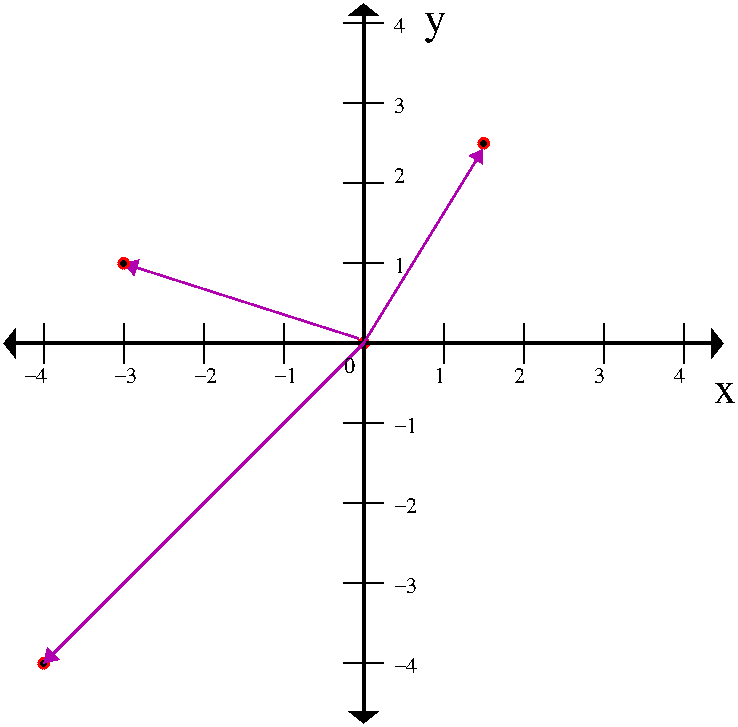
\includegraphics[height=6cm]{../Figures/2DGrid_plus_vector.png}
\end{center}

\end{frame}

\begin{frame}
\frametitle{Notation}
For reasons that will become clear we describe them as columns rather than rows.
\pause
\begin{equation}
\vd{1.1}{2.5}, \vd{-3.7}{0.34} 
\end{equation}


 
\pause
As variables we use the following notation
\begin{equation}
\v{v} = \vd{-4.67}{0.76}
\end{equation}

\end{frame}

\begin{frame}
\frametitle{Notation contd.}

In textbooks you will also see the following alternatives ....
\[
\mathbf{v}\;\; , \;\; \vec{v}
\]
they all mean the same thing - a vector !

\pause
If we want a vector in row form then there is an explicit operation to get that.

\begin{equation}
\v{v}^\intercal = \vdt{-4.67}{0.76} 
\end{equation}

\end{frame}

\survey{https://moodle.royalholloway.ac.uk/mod/quiz/view.php?id=462536}


\end{document}
